\section{Human Interfaces}

There are multiple human interface components on the Thetis board, as shown in \Fref{fig:revision_f5_hid}.

\begin{figure}[h!]
    \centering
    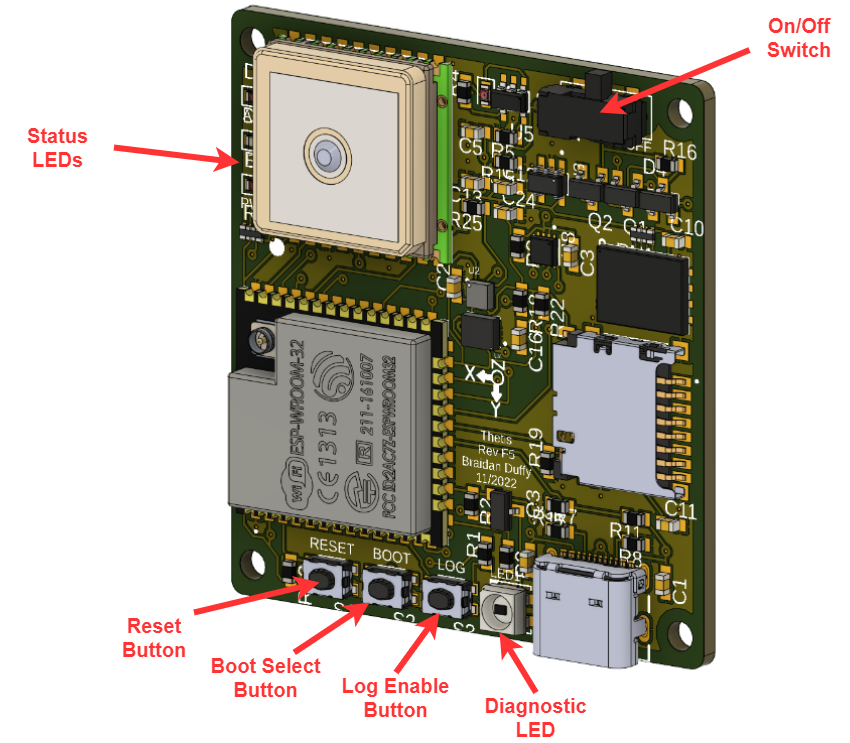
\includegraphics[height=3.5in]{revision_f5_hid.png}
    \caption{Thetis Revision F5 with callouts for human interface components}
    \labfig{revision_f5_hid}
\end{figure}

\subsection{Buttons} \label{sec:buttons}
Along the bottom edge are three buttons: reset, boot select, and log enable.

\begin{description}
    \item[The reset button] will perform a power-on reset of the microcontroller when pressed, restarting the firmware and clearing any errors.
    \item[The boot select button] will put the microcontroller into the bootloader (safe/programming) mode if pressed during a reset or power cycle. 
    \item[The log enable button] will start or stop logging when pressed for half of a second. The current logging status is shown by the LEDs. 
\end{description}

\subsection{Primary \acs{RGB} \acsp{LED}}
\label{sec:led}

The main diagnostic \ac{RGB} \ac{LED} indicates the mode and status of Thetis using different colors and flashing behaviors.

\newcommand{\ledFigure}[3]{
    \begin{figure}[H]
        \centering
        \includegraphics[width=0.5\textwidth]{LEDs/#1.png}
        \caption{#2}
        \label{fig:#3}
    \end{figure}
}

\newcommand{\ledBlinkFigure}[6]{
    \begin{figure}[H]
        \centering
        \subfloat[#2]{\includegraphics[width=0.45\textwidth]{LEDs/#1.png} \label{subfig:#6_#1}} \hskip3ex
        \subfloat[#4]{\includegraphics[width=0.45\textwidth]{LEDs/#3.png} \label{subfig:#6_#2}}
        \caption{#5}
        \label{fig:#6}
    \end{figure}
}

\subsubsection{Booting (Purple)}

A steady purple \ac{LED}, as shown in \Fref{fig:booting_led} indicates that Thetis is switched on and booting.

\ledFigure{purple}{a steady purple \acs{LED} indicating that Thetis is switched on and booting}{booting_led}

\subsubsection{Standby (Yellow)}

An steady yellow \ac{LED}, as shown in \Fref{fig:standby_led} indicates that Thetis is switched on and in standby mode. 
This mode is active until the device passes a self-test, its sensors report that they are calibrated, and the fusion algorithm is online and stable.
Currently, this mode is bypassed and ignored.

\ledFigure{yellow}{A steady yellow \acs{LED} indicating that Thetis is switched on and in standby mode}{standby_led}

\subsubsection{Ready, No GPS (Blue)}

A blinking (once per second) blue \ac{LED}, as shown in \Fref{fig:ready_no_gps_led} indicates that Thetis is online, calibrated, and ready to start logging.
However, it has not yet acquired a GPS fix.
This mode will still allow logging, but the position messages will either not be populated or not accurate.

% \ledBlinkFigure{blue}{The \ac{LED} is blue for approximately 1 second}{off}{Then turns off for one second}{A blinking blue \ac{LED} indicating that Thetis is switched on and ready to log data without a GPS fix}{ready_no_gps_led}

\begin{figure}[H]
    \centering
    \subfloat[The \ac{LED} is blue for approximately 250 milliseconds]{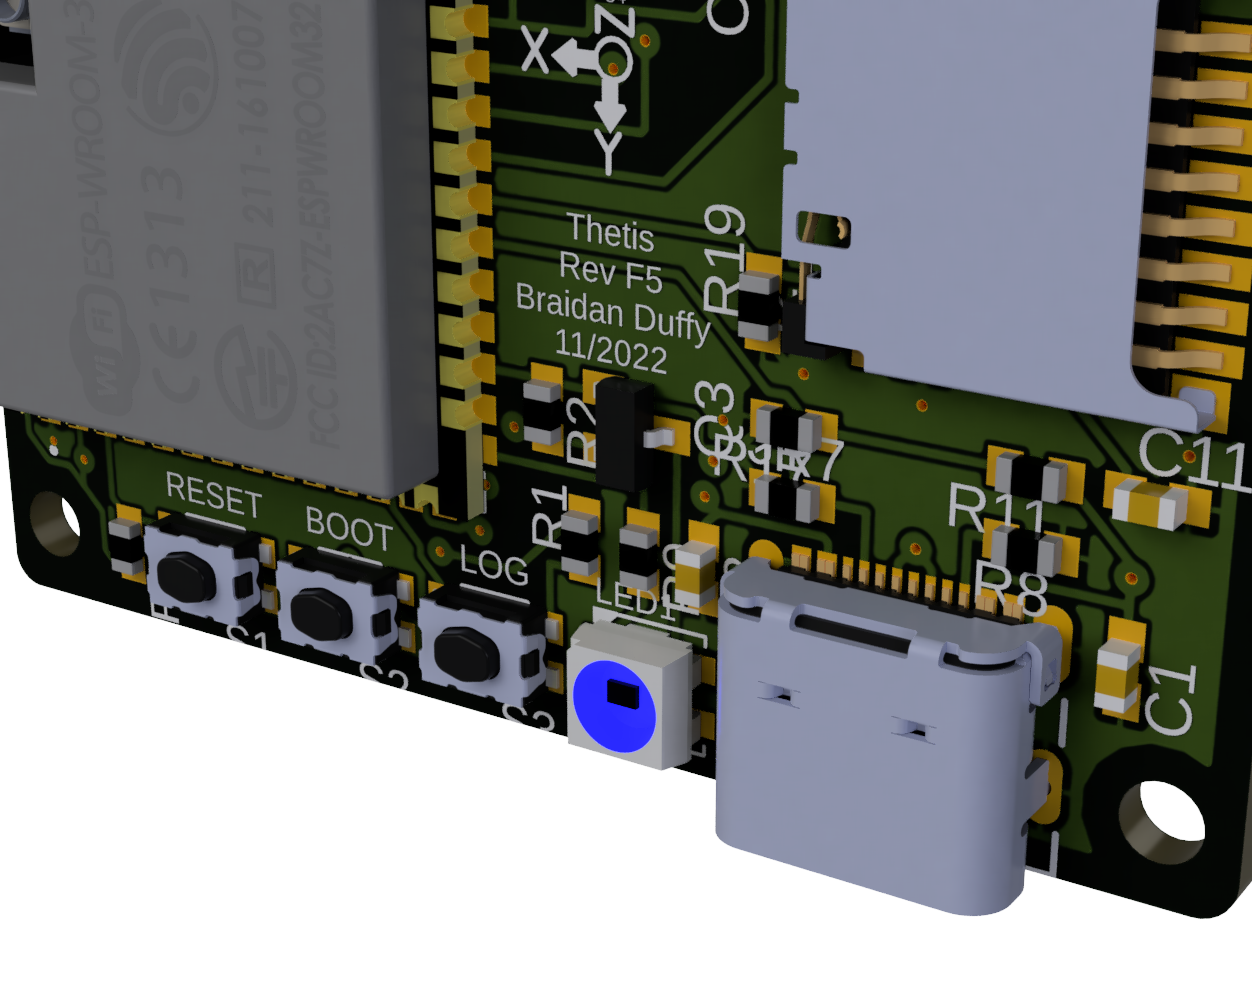
\includegraphics[width=0.45\textwidth]{LEDs/blue.png} \label{subfig:ready_no_gps_led_blue}} \hskip3ex
    \subfloat[Then turns off for 250 milliseconds]{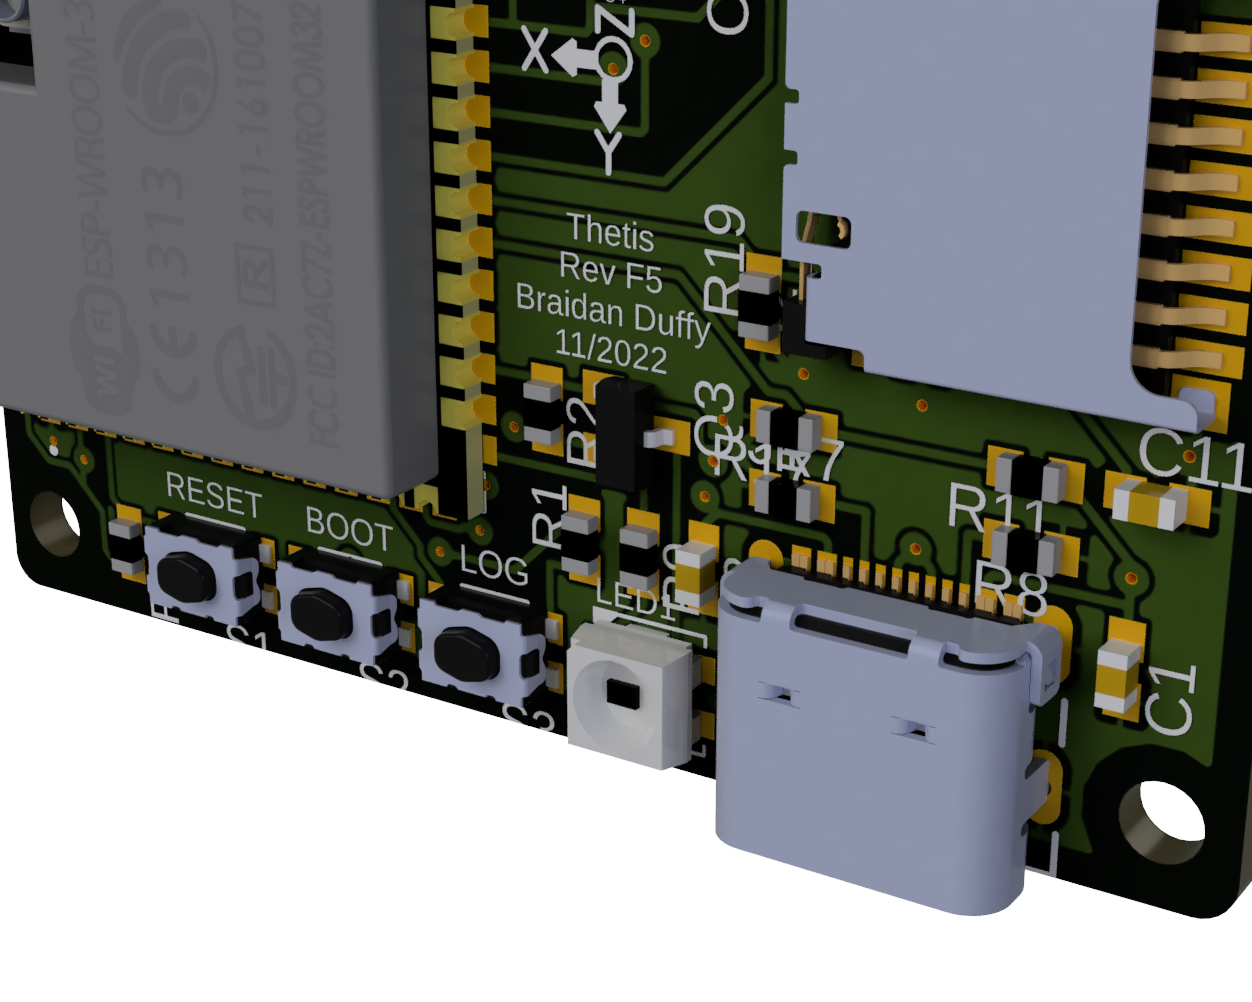
\includegraphics[width=0.45\textwidth]{LEDs/off.png} \label{subfig:ready_no_gps_led_off}}
    \caption{A blinking blue \ac{LED} indicating that Thetis is switched on and ready to log data without a GPS fix}
    \label{fig:ready_no_gps_led}
\end{figure}

\subsubsection{Logging, No GPS (Blue)}

A steady blue \ac{LED}, as shown in \Fref{fig:logging_no_gps_led} indicates that Thetis is switched on and logging data without a GPS fix.
This mode will still log data as expected, but the position messages will either not be populated or not accurate.

\ledFigure{blue}{A steady blue \acs{LED} indicating that Thetis is switched on and logging without a GPS fix}{logging_no_gps_led}

\subsubsection{Ready, GPS (Green)}

A blinking (once per second) green \ac{LED}, as shown in \Fref{fig:ready_gps_led} indicates that Thetis is online, calibrated, and ready to start logging with a valid GPS fix.
This will populate the position message with reasonably-accurate GPS data.

% \ledFigure{ready_gps_led}{A blinking green \acs{LED} indicating that Thetis is switched on and ready to log data with a GPS fix}

\begin{figure}[H]
    \centering
    \subfloat[The \ac{LED} is green for 250 milliseconds]{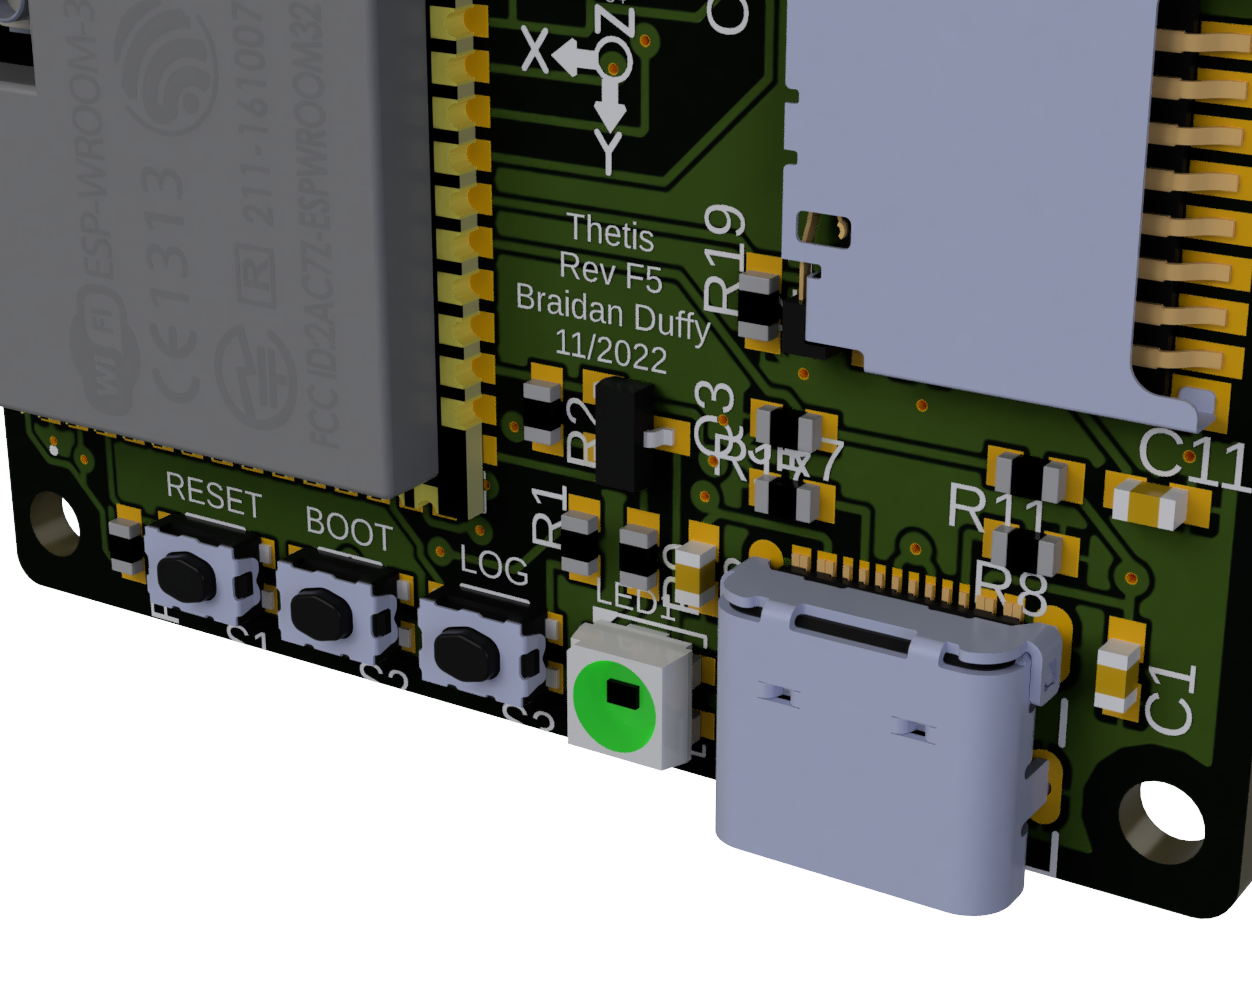
\includegraphics[width=0.45\textwidth]{LEDs/green.png} \label{subfig:ready_gps_led_green}} \hskip3ex
    \subfloat[Then turns off for 250 milliseconds]{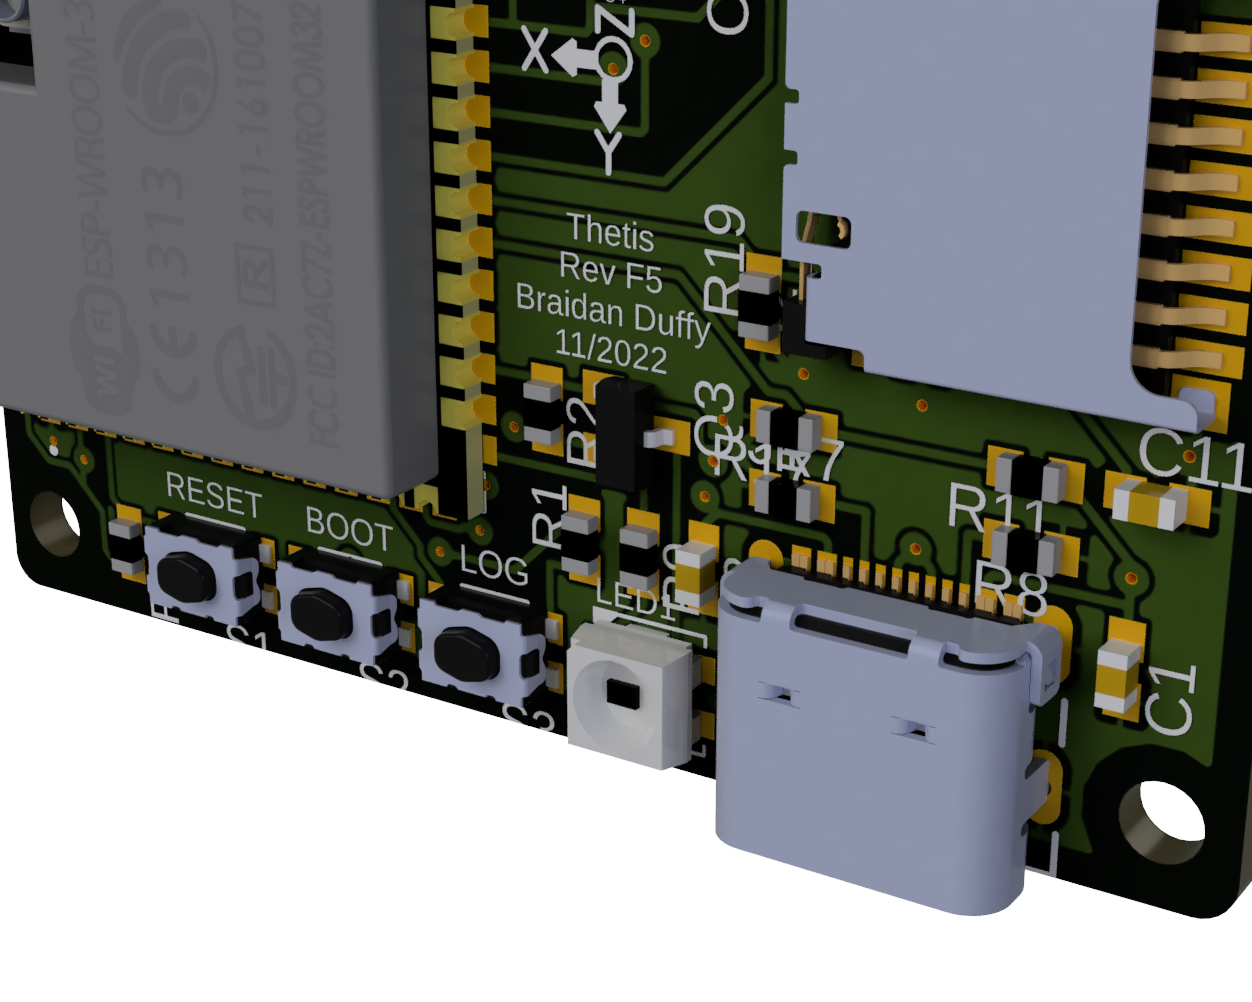
\includegraphics[width=0.45\textwidth]{LEDs/off.png} \label{subfig:ready_gps_led_off}}
    \caption{A blinking green \ac{LED} indicating that Thetis is switched on and ready to log data with a GPS fix}
    \label{fig:ready_gps_led}
\end{figure}

\subsubsection{Logging, GPS (Green)}

A steady green \ac{LED}, as shown in \Fref{fig:logging_gps_led} indicates that Thetis is switched on and logging data with a GPS fix.
Position messages will be populated with reasonably-accurate GPS data in this mode.

\ledFigure{green}{A steady green \acs{LED} indicating that Thetis is switched on and logging with a GPS fix}{logging_gps_led}

\subsubsection{Error (Red and Yellow)}

When Thetis enters an error state, the main \acs{RGB} \ac{LED} will begin flashing red and yellow error codes based on the error type.
The red blinks will precede the yellow blinks and there will be a short interval between code flashes.
In the error state, Thetis will lock up and lose all functionality until the battery dies.
The device will require a full power cycle or reset to clear the error code.
In-depth diagnostic information may be available if data is being streamed to a host computer through the USB port and serial monitor terminal (e.g. PuTTY).

\begin{figure}[H]
    \centering
    \subfloat[The \ac{LED} is red with 250 millisecond blinks for a certain number of times]{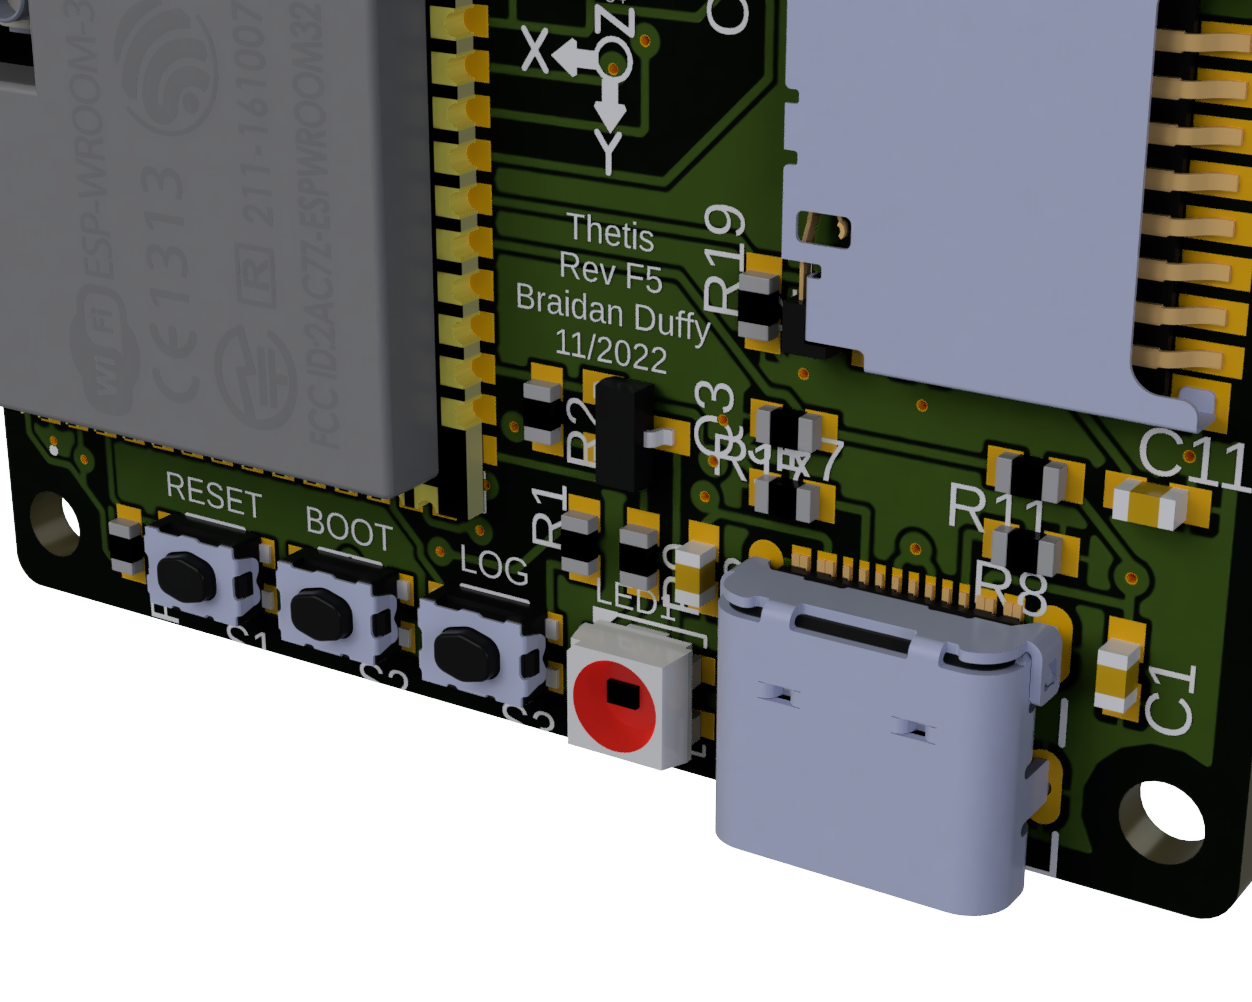
\includegraphics[width=0.3\textwidth]{LEDs/red.png} \label{subfig:error_green}} \hskip3ex
    \subfloat[Then turns yellow with 250 millisecond blinks for a certain number of times]{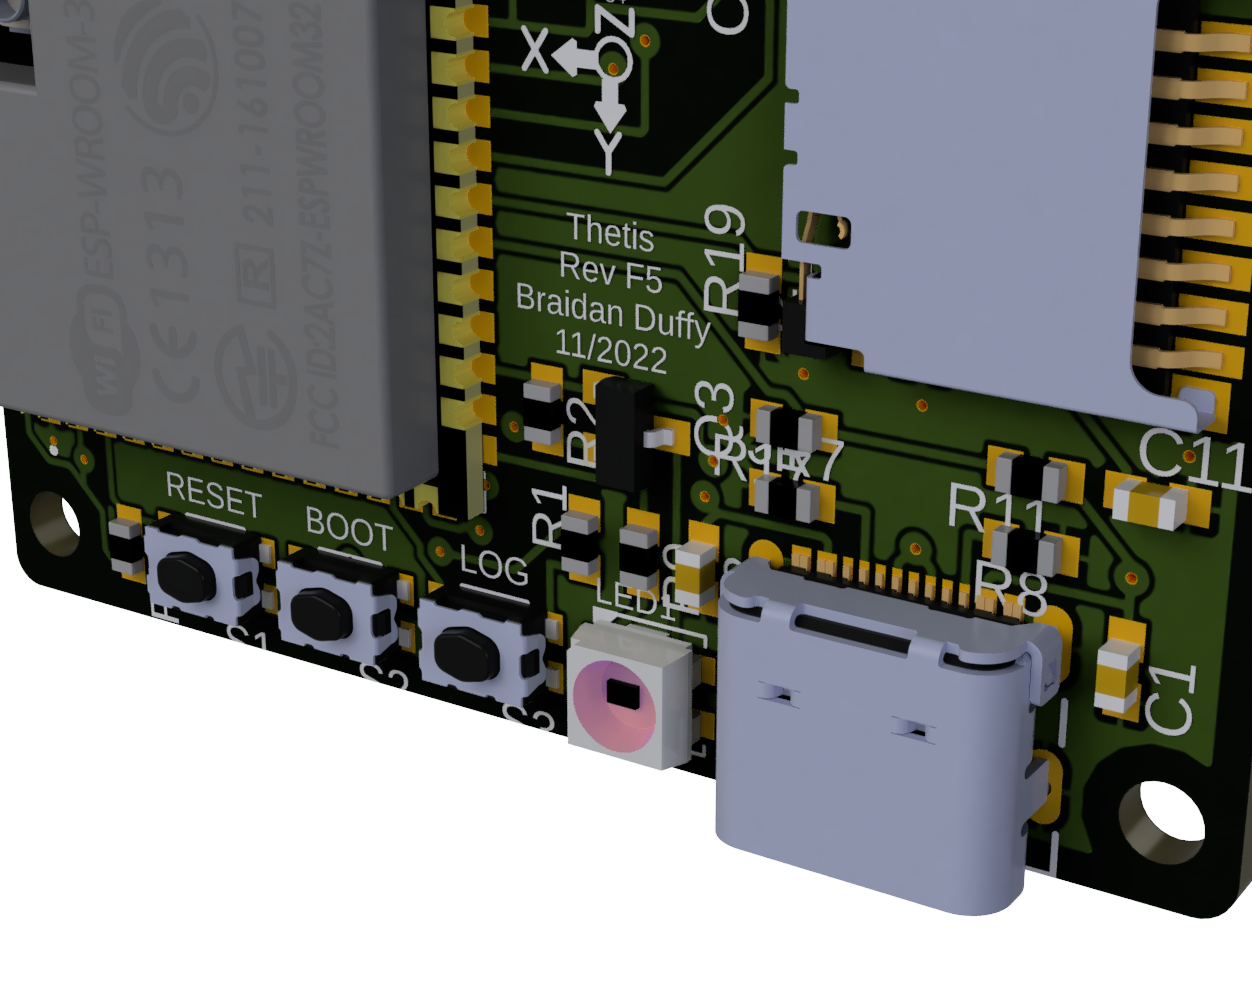
\includegraphics[width=0.3\textwidth]{LEDs/yellow.png} \label{subfig:error_yellow}} \hskip3ex
    \subfloat[Then turns off for one second]{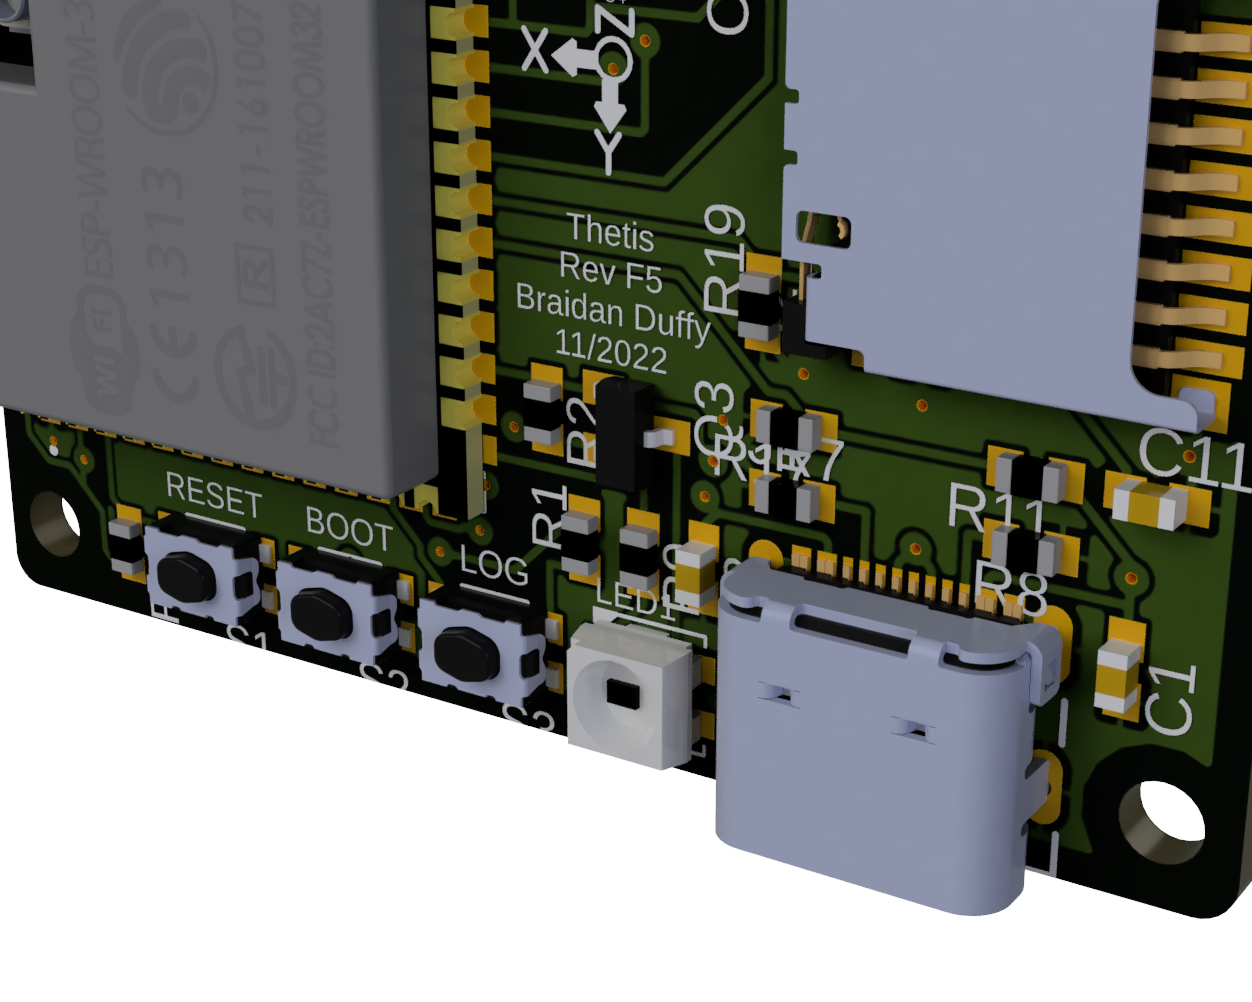
\includegraphics[width=0.3\textwidth]{LEDs/off.png} \label{subfig:error_off}}
    \caption{A blinking red and yellow \ac{LED} indicates that Thetis is switched on and in an error state according to \Fref{tab:error_codes}}
    \label{fig:error}
\end{figure}

\customTable
{l c c m{0.5\textwidth}}
{Error & Red & Yellow & Description}
{
    General & 1 & 1 & General failure state; unhandled or unknown error \\
    Settings & 1 & 2 & Board is initialized with or encounters invalid settings \\
    Low Battery & 2 & 1 & Battery voltage is below the threshold limit and the system has not automatically shutdown \\
    Battery Monitor & 2 & 2 & The battery monitoring \acs{IC} fails to initialize \\
    Temperature & 2 & 3 & The reported system temperature exceeds a threshold\tablefootnote{not currently implemented} \\
    Card Mount & 3 & 1 & The data log filesystem fails to mount to the \acs{microSD} card \\
    Card Type & 3 & 2 & The data log filesystem initializes, but reports an incorrect \acs{microSD} card type or format \\
    File Operations & 3 & 3 & A requested filesystem operation fails to execute \\
    Wi-Fi Radio & 4 & 1 & The Wi-Fi radio fails to initialize or encounters errors \\
    BlueTooth Radio & 4 & 2 & The BlueTooth radio fails to initialize or encounters errors\footnotemark[\value{footnote}] \\
    \acs{GPS} Radio & 4 & 3 & The \acs{GPS} radio fails to initialize or encounters an error \\
    \acs{IMU} & 5 & 1 & The \acs{IMU} fails to initialize or encounters an error \\
    Magnetometer & 5 & 2 & The magnetometer fails to initialize or encounters an error \\
    Fusion & 5 & 3 & The sensor fusion algorithm encounters an error\footnotemark[\value{footnote}] \\
    CANbus & 6 & 1 & The CANbus transceiver fails to initialize or encounters an error\footnotemark[\value{footnote}] \\
    Device ID & 6 & 2 & The device ID is not properly configured\footnotemark[\value{footnote}] \\
}
{Thetis error code table}
{tab:error_codes}

\subsubsection{User control}

The on-board \ac{RGB} \ac{LED} can be controlled by the user using the strobe and colour commands.  
See \Fref{sec:strobeCommand} and \Fref{sec:colourCommand} for more information.

\subsection{Secondary Diagnostic \acs{LED}}
In addition to the main \ac{RGB} \ac{LED}, Thetis also has four other monochromatic diagnostic \acp{LED} on the left and top edge of the board.
From top to bottom, these \acp{LED} are for battery charging, activity, GPS fix, and power.
Their locations are highlighted in \Fref{fig:diagnostic_led}

\ledFigure{diagnostic}{Additional monochromatic diagnostic LEDs present on Thetis}{diagnostic_led}

\begin{description}
    \item[The battery charging \ac{LED}] illuminates orange when the battery is plugged in, \ac{USB} is connected, and the battery is not at 4.2V. The board does not need to be on to charge the battery.
    \item[The activity \ac{LED}] is blue and typically only illuminated when the device is logging. This behavior can be changed in the firmware.   
    \item[The \acs{GPS} fix \ac{LED}] blinks red once per second when the GPS is acquiring a signal. Once the signal is acquired, it blinks quickly once every 15 seconds.
    \item[The power \ac{LED}] illuminates red when the 3V3 bus on the board is active; nominally when the battery or \ac{USB} is plugged in and the switch turned on.
\end{description}
